\documentclass[12pt]{article}
\usepackage{amsmath, graphicx}
\usepackage{tikz}
\usepackage[colorlinks=true, allcolors=black]{hyperref}
\usepackage{hyperref}
\usepackage[french]{babel}
\usepackage[top=2.3cm, bottom=2.3cm, left=2.5cm, right=2.5cm]{geometry}

\begin{document}

\begin{titlepage}
    \begin{center}
        \vspace*{1cm}
            
        \Huge
        \textbf{GPTeirb: une méthode de génération de texte sans paramètres utilisant des compresseurs}
            
        \vspace{1.2cm}
        \Large
        %Traitement de l'information
            
        
        \hrule
        \vspace{0.5cm}
        \textbf{Léo Paillé - Gatien Menaud - Alix Renoncourt}
        \vspace{0.5cm}
        \hrule
            
        \vspace{1cm}

        \large
        EI5IS102 - Traitement de l’Information\\
        Département informatique\\
        S5 - 2023/2024

        \vspace{1cm}

        
\includegraphics[width=0.5\textwidth]{./assets/logo.png}
        \vfill
        
        \vspace{0.5cm}
            
        
\includegraphics[width=0.4\textwidth]{./assets/Logo_enseirb.png}
        
    \end{center}
    
        \small
        ENSEIRB-MATMECA, Bordeaux, 10 Janvier 2024
        \normalsize
            
\end{titlepage}

\large
\tableofcontents
\normalsize

\newpage

\section{Introduction}
Dans ce rapport, nous allons décrire le projet que nous avons décidé de réaliser. Il s'agit du traitement d'un jeu de données publiques issues de Kaggle, ainsi que de la création d'un modèle de génération de texte. Nous avons d'abord formaté les données pour créer des exemples d'entraînement, puis nous avons utilisé une approche nouvelle basée sur KNN et gzip dans le but de générer du texte. Cette approche se base sur l'article “Low-Resource” Text Classification: A Parameter-Free Classification Method with Compressors\cite{jiang-etal-2023-low} et utilise le moyen de classification à la place d'un transformeur génératif pré-entraîné pour sélectionner le prochain token.\\

Cette méthode de traitement de données est semblable aux modèles de génération de texte par intelligence artificielle, tels que ChatGPT développé par la société OpenAI.\\
Notre code est disponible à \href{https://github.com/Leikoe/gpt-eirb}{https://github.com/Leikoe/gpt-eirb}.

\section{Présentation des données}
Pour créer un modèle capable de générer du texte à partir d'un mot ou d'une phrase (appelé \textit{prompt}), il est tout d'abord nécessaire de l'entraîner à partir de texte préexistant. Nous avons décidé pour cela de récupérer un jeu de données \textit{TinyStories.txt\cite{eldan2023tinystories}} (une fois décompressé), contenant plusieurs histoires de quelques lignes, en anglais, totalisant plus de 1.6G de caractères. Notez qu'une partie non négligeable de ces textes a été elle-même générée par les modèles GPT-3.5 et GPT-4. Voici un échantillon du jeu de données en figure \ref{fig:echantTS} : 

\begin{figure}[h]
	\centering
    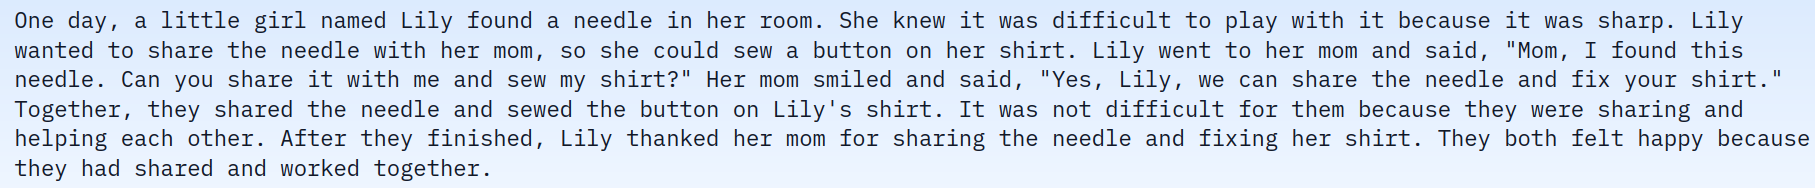
\includegraphics[scale=0.26]{assets/EchantillonTinyStories.png}
    \caption{\textit{Échantillon de TinyStories.txt}}
    \label{fig:echantTS}
\end{figure}

\newpage

\section{Présentation de la méthode}
L'objectif étant de générer du texte, notre modèle doit être capable de déterminer le token (ici un caractère) suivant d'une suite de tokens. Comme dans le papier original, le but est de classifier du texte, c'est-à-dire des d'échantillons de phrases (suites de tokens). Les classes sont tous les tokens possibles (comme pour un transformeur génératif). Nous avons choisi ici les caractères du texte d'entraînement.


\subsection{Création des exemples}
Un exemple est un couple \textit{(contexte, cible)}. Pour créer un de ces couples, nous générons un entier aléatoire que nous utilisons comme offset dans le texte de base, puis nous récupérons les \textit{context\_size} tokens suivants. 

\begin{figure}[h]
	\centering
    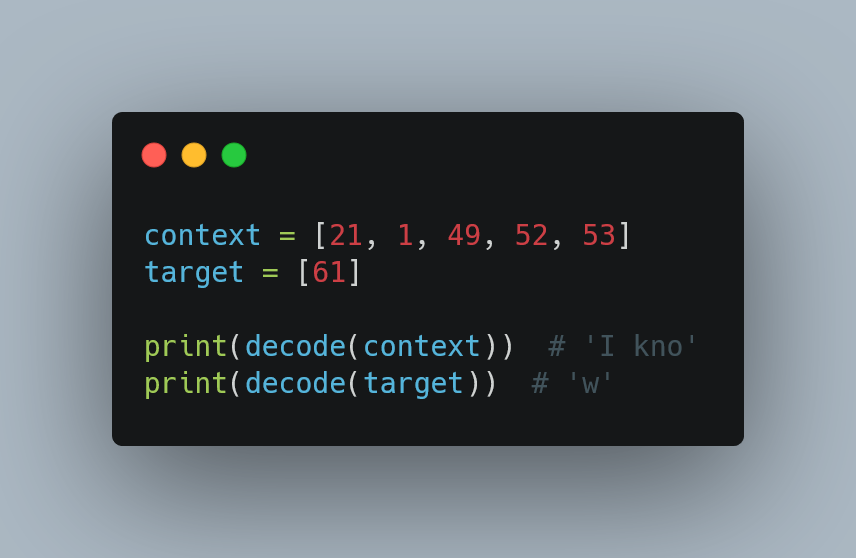
\includegraphics[scale=0.4]{assets/context_target.png}
    \caption{\textit{Un exemple d'entraînement}}
    \label{fig:training_example_example}
\end{figure}

\subsection{Création du modèle}
Pour créer le modèle, nous devons calculer une matrice de NCD (distances de compression normalisées). Chaque ligne de cette matrice est un vecteur qui correspond à un exemple d'entraînement. Le vecteur des NCD de cette ligne est calculé à partir des NCD entre l'exemple et tous les autres exemples.

On obtient donc une matrice de taille N*N où N est le nombre d'exemples.\\

\begin{center}
    
    \fbox{\begin{tikzpicture}[scale=0.8]
      \foreach \y [count=\n] in {
          {22, 87, 92, 14, 53},
        } {

          % heatmap tiles
          \foreach \x [count=\m] in \y {
            \node[fill=red!\x!yellow, minimum size=6mm, text=white] at (\m,-\n) {\x};
          }
        }
    
      % row labels
      \foreach \a [count=\i] in {I am a} {
        \node[minimum size=6mm] at (-1,-\i) {\a};
      }
      % column labels
      \foreach \a [count=\i] in {[Hello] World, [The] man,[A] woman, [NNs] are, [I eat] apples} {
        \node[minimum size=6mm, rotate=90] at (\i,1.5) {\a};
      }
    
    \end{tikzpicture}}
    
    ~\\~\textbf{ Exemple d'un vecteur de NCD}
    
\end{center}

On peut observer que les suites de tokens avec un sens proche (et donc un token cible suivant logique) obtiennent un score plus élevé lors du calcul de la NCD. \\
Ici, nous pourrions sélectionner "man" ou "woman" comme prochain token pour le prompt "I am a". \\

Pour cela, nous allons récupérer \textit{n\_train} échantillons, puis à partir de chacun, générer \textit{context\_size} exemples. 
Pour chaque exemple, nous allons calculer un vecteur de NCD vers tous les autres exemples. Ce calcul est très lent et nous avons donc dû effectuer les compressions par batch sur GPU. Pour cela, nous avons utilisé nvCOMP\cite{nvcomp}, la librairie de compression propriétaire de NVIDIA. Cependant, cette librairie est en C++, et les seuls bindings à jour en python sont disponibles dans la librairie kvikio \cite{kvikio} de la suite RAPIDS\cite{rapidsai} de NVIDIA. 

\subsection{Optimisations du calcul de la matrice de NCDs}
Nous avons seulement besoin des tailles compressées des exemples et avons donc modifié la fonction de compression par batch de kivikio\cite{kvikio}. Après avoir mesuré le code, nous nous sommes aperçus que la majorité du temps était passé à copier chacun des strings vers la mémoire du GPU. Nous avons donc copié à la suite dans un buffer tous les strings de chaque groupe (\textit{batch}), pour copier le buffer en une seule opération sur le gpu. Cela a grandement accéléré la génération du modèle.


\subsection{Utilisation du modèle}
Une fois que nous avons obtenu notre matrice correspondant à notre modèle, il est simple et rapide de faire générer du texte par un programme prenant en entrée un prompt écrit par l'utilisateur, ainsi que notre modèle, et générant en sortie du texte. Ce texte se développe alors, token par token de la manière suivante :\\
- On récupère les $max(taille\_prompt$, $context\_size)$ derniers caractères du contexte (le prompt suivi du texte généré jusque là)\\
- On calcule le vecteur de NCDs pour les $context\_size$ derniers tokens du contexte. Cela donne une liste de flottants de longueur \textit{n\_train}\\
- On utilise un KNN pour trouver les lignes les plus proches du contexte actuel.\\
- On sélectionne le token suivant comme la classe prédite par le KNN\\
- On rajoute le nouveau token à la suite du contexte\\
- On réitère l'opération jusqu'à qu'une condition d'arrêt soit satisfaite (fin de phrase, nombre de caractères requis par l'utilisateur atteint, arrêt forcé...)\\

\section{Analyse du modèle et des résultats}
Nous observons une génération médiocre, sans réel sens. Cela peut être dû à plusieurs raisons, 

Premièrement, le compresseur utilisé est l'implémentation GPU de LZ4. Celui-ci ne possède pas un très bon facteur de compression contrairement à l'implémentation CPU de GZIP (celui par défaut en python). Cela influe très fortement sur les tailles compressées des exemples. Ici on observe que tous les exemples pour un $context\_size$ entre 4 et 16 ont une taille compressée tournant autour de 260 octets, ce qui rend très difficile pour le KNN de faire la différence entre les divers exemples.

Deuxièmement, nous avons utilisé un $tokinizer$ de niveau caractère. Nous obtiendrons probablement de meilleurs résultats avec un $tokenizer$ basé sur SentencePiece \cite{kudo2018sentencepiece}. Cela aiderait énormément la qualité de génération pour des petites valeurs de $context\_size$.

Troisièmement, l'approche utilisée ne s'échelonne pas bien. La taille du modèle est quadratique par rapport à la taille des données sur lesquelles il est entraîné. Cela devient vite bien trop grand, peut-être qu'un gigantesque modèle de cette architecture parviendrait à formuler des phrases.


\section{Conclusion}

Ce travail nous a permis de mettre en pratique des connaissances en programmation Python, mais aussi en traitement d'informations. Nous avons pu manipuler un grand corpus de données textuelles non labellisées afin de créer un modèle, permettant par la suite de générer du texte. Nous n'avons cependant pas pu atteindre cet objectif dans son entièreté, notamment par manque de ressources numériques, telles que de la puissance de calcul et de l'espace mémoire.

Nous avons tout de même pu approfondir nos connaissances, à la fois dans l'écriture du code, que dans les recherches qui nous ont permis de le réaliser. Nous avons pu utiliser divers outils mis à notre disposition depuis le web, en se basant plus particulièrement sur des projets communautaires ayant déjà traité ce sujet et des vidéos abordant le thème \cite{karpathy2021lets}. Pour conclure, le développement de l'intelligence artificielle est un enjeu majeur dans le monde du numérique d'aujourd'hui, surtout en ce qui concerne les discussions textuelles, et nous avons pu profiter de ce projet pour tenter de créer notre propre modèle de langage, nous permettant d'explorer en profondeur et d'en apprendre davantage sur ce sujet.\\

\section{Références}
\bibliographystyle{plain}
\bibliography{refs}

\end{document}